\documentclass{article}

\usepackage{tikz}
\usepackage{subcaption}
\usepackage{listings}

\begin{document}
\pagestyle{empty}

\def\layersep{3.5cm}

\section{Task 2}

\subsection{Problem Description}
Instead of trying to find the minimum of the Rosenbrock's function in task 1, we would like to solve the "exclusive or" (xor) problem in task 2. The problem exists out of two input bits which should produce their associated value of the (only) output bit. Please see Table~\ref{tab:tt} for the truth table.

\begin{table}[!h]
	\centering
	\begin{tabular}{| l | c | r |}
		\hline
		$x_1$ & $x_2$ & $y$ \\ \hline
		0 & 0 & 0 \\ \hline
		0 & 1 & 1 \\ \hline
		1 & 0 & 1 \\ \hline
		1 & 1 & 1 \\ \hline
	\end{tabular}
	\caption{The truth table. When only one of the two input bits is true, the output bit should be true.}
	\label{tab:tt}
\end{table}

A perceptron cannot solve this problem, because the classes (different values of y) could not be separated linearly with one line in twodimensional space. Please see Figure~\ref{fig:sep} why. 

\begin{figure}[!h]
	\centering
	\begin{subfigure}[b]{0.3\textwidth}
		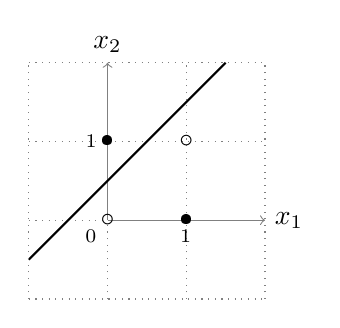
\begin{tikzpicture}[x=1cm,y=1cm]
			\draw[latex-latex, thin, draw=gray, ->] (0,0)--(2,0) node [right] {$x_1$};
			\draw[latex-latex, thin, draw=gray, ->] (0,0)--(0,2) node [above] {$x_2$}; 
			\draw[thick] (-1, -0.5)--(1.5, 2); 

			\draw [dotted, gray] (-1, -1) grid (2, 2);
			\node [black] at (0, 1) {\textbullet};
			\node [black] at (-0.2, 1) {$_1$};
			\node [black] at (1, 0) {\textbullet};
			\node [black] at (1, -0.2) {$_1$};
			\node [black] at (0, 0) {$\circ$} node [below left] {$_0$};
			\node [black] at (1, 1) {$\circ$};
		\end{tikzpicture}
		\caption{}
	\end{subfigure}
	\begin{subfigure}[b]{0.3\textwidth}
		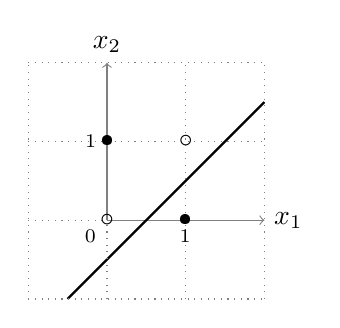
\begin{tikzpicture}[x=1cm,y=1cm]
			\draw[latex-latex, thin, draw=gray, ->] (0,0)--(2,0) node [right] {$x_1$};
			\draw[latex-latex, thin, draw=gray, ->] (0,0)--(0,2) node [above] {$x_2$}; 
			\draw[thick] (-0.5,-1)--(2, 1.5);

			\draw [dotted, gray] (-1, -1) grid (2, 2);
			\node [black] at (0, 1) {\textbullet};
			\node [black] at (-0.2, 1) {$_1$};
			\node [black] at (1, 0) {\textbullet};
			\node [black] at (1, -0.2) {$_1$};
			\node [black] at (0, 0) {$\circ$} node [below left] {$_0$};
			\node [black] at (1, 1) {$\circ$};
		\end{tikzpicture}
		\caption{}
	\end{subfigure}
	\begin{subfigure}[b]{0.3\textwidth}
		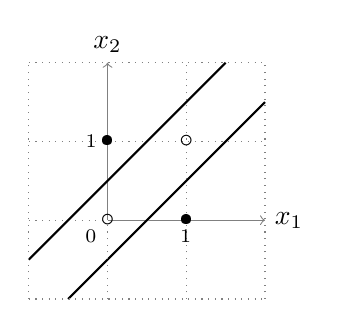
\begin{tikzpicture}[x=1cm,y=1cm]
			\draw[latex-latex, thin, draw=gray, ->] (0,0)--(2,0) node [right] {$x_1$};
			\draw[latex-latex, thin, draw=gray, ->] (0,0)--(0,2) node [above] {$x_2$}; 
			\draw[thick] (-1, -0.5)--(1.5, 2); 
			\draw[thick] (-0.5,-1)--(2, 1.5);

			\draw [dotted, gray] (-1, -1) grid (2, 2);
			\node [black] at (0, 1) {\textbullet};
			\node [black] at (-0.2, 1) {$_1$};
			\node [black] at (1, 0) {\textbullet};
			\node [black] at (1, -0.2) {$_1$};
			\node [black] at (0, 0) {$\circ$} node [below left] {$_0$};
			\node [black] at (1, 1) {$\circ$};
		\end{tikzpicture}
		\caption{}
	\end{subfigure}
	\caption{3 trials to seperate the classes. The filled circles are true cases and the empty circles are false cases.}
	\label{fig:sep}
\end{figure}

As seen in Figure~\ref{fig:sep} (c) it is possible to solve the xor problem, but not with a perceptron. We need something advanced, like a neural network.

\begin{figure}[h]
	\begin{tikzpicture}[shorten >=1pt,->,draw=black!50, node distance=\layersep]
	   	\tikzstyle{every pin edge}=[<-,shorten <=1pt]
		\tikzstyle{neuron}=[circle,fill=black!25,minimum size=17pt,inner sep=0pt]
		\tikzstyle{input neuron}=[neuron, fill=green!50];
		\tikzstyle{output neuron}=[neuron, fill=red!50];
	   	\tikzstyle{hidden neuron}=[neuron, fill=blue!50];
		\tikzstyle{annot} = [text width=4em, text centered]

		% Draw the input layer nodes
		\node[input neuron, pin=left:$x_1$] (I-1) at (0,-1) {};
		\node[input neuron, pin=left:$x_2$] (I-2) at (0,-3) {};

		\path node[hidden neuron] (H-1) at (\layersep,-1 cm) {};
		\path node[hidden neuron] (H-2) at (\layersep,-3 cm) {};

	    	% Draw the output layer node %[yshift=0.5cm]
	    	\node[output neuron,pin={[pin edge={->}]right:y}, right of=H-1, yshift=-1.0cm] (O) {};

		% Connect every node in the input layer with every node in the
		% hidden layer.
		\path (I-1) edge node [above] {$w1$} (H-1) ;
		\path (I-1) edge node [pos=0.75, below, sloped] {$w3$} (H-2);
		\path (I-2) edge node [pos=0.75, above, sloped] {$w2$} (H-1);
		\path (I-2) edge node [below] {$w4$} (H-2);

		% Connect every node in the hidden layer with the output layer
		\path (H-1) edge node [above, sloped] {$w5$} (O);
		\path (H-2) edge node [below, sloped] {$w6$} (O);

		% Annotate the layers
		\node[annot,above of=H-1, node distance=1cm] (hl) {Hidden layer};
		\node[annot,left of=hl] {Input layer};
		\node[annot,right of=hl] {Output layer};
	\end{tikzpicture}
	\caption{The xor neural network.}
	\label{fig:nn}
\end{figure}

\subsection{Solution}
We made a multilayer neural network with three nodes and six weights \footnote{The network could be trained much faster when bias nodes are used, but in sight of the assignment there is chosen to do it the hard way and make the problem more difficult.}. Please see Figure~\ref{fig:nn} for an illustration. The network is trained with the data of the truth table and the weights are updated with the algorithms of task 1. The algorithms tries to steer the weights in such a way the errors of the predicted classes and the actual classes are minimized.

\begin{figure}[h]
	\begin{lstlisting}[language=matlab, numbers=left, tabsize=4, frame=single, basicstyle=\footnotesize]
	function [y] = xornet(x1, x2, w)
		net1 = w(1) * x1 + w(2) * x2;
	 	y1 = phi(net1);
		net2 = w(3) * x1 + w(4) * x2;
	 	y2 = phi(net2);
		net = w(5) * y1 + w(6) * y2;
	 	y = phi(net);
	end
	\end{lstlisting}
	\caption{The computation of the output value, based on the input values and the weights.}
\end{figure}

\begin{figure}
	\begin{lstlisting}[language=matlab, numbers=left, tabsize=4, frame=single, basicstyle=\footnotesize, breaklines=true]
function [d] = mysse(w)
	d = power(xornet(0, 0, w) - 0, 2) + 
		power(xornet(0, 1, w) - 1, 2) + 
		power(xornet(1, 0, w) - 1, 2) + 
		power(xornet(1, 1, w) - 0, 2);
end
	\end{lstlisting}
	\caption{The computation of the sum squared error of the weights.}
\end{figure}


\begin{figure}
	\begin{lstlisting}[language=matlab, numbers=left, tabsize=4, frame=single, basicstyle=\footnotesize, breaklines=true, deletekeywords={input}]
function [d] = dmysse(w)
	d = zeros(1, 6);

	input = [0, 0; 0, 1; 1, 0; 1, 1];
	target = [0, 1, 1, 0];

	for i = 1:4
		net1 = w(1) * input(i, 1) + w(2) * input(i, 2);
		y1 = phi(net1);
		net2 = w(3) * input(i, 1) + w(4) * input(i, 2);
		y2 = phi(net2);
		net = w(5) * y1 + w(6) * y2; 
		y = phi(net);
	
		d(1) = d(1) + (y - target(i)) * phiprime(net) * w(5) * phiprime(net1) * input(i, 1);
		d(2) = d(2) + (y - target(i)) * phiprime(net) * w(5) * phiprime(net1) * input(i, 2);
		d(3) = d(3) + (y - target(i)) * phiprime(net) * w(6) * phiprime(net2) * input(i, 1);
		d(4) = d(4) + (y - target(i)) * phiprime(net) * w(6) * phiprime(net2) * input(i, 2);
		d(5) = d(5) + (y - target(i)) * phiprime(net) * y1;
		d(6) = d(6) + (y - target(i)) * phiprime(net) * y2;
	end
	d = d * 2;
end
	\end{lstlisting}
	\caption{The computation of the derivatives of the sum squared error of the weights.}
\end{figure}

\begin{figure}
	\centering
	\begin{eqnarray}
	 \phi(x) & = & \frac{1}{1 + e^{-x}} \\
	   \phi'(x) & = & \phi(x)(1 - \phi(x))
	\end{eqnarray}
	\caption{The sigmoid function (1) and the derivative (2).}
\end{figure}

\begin{figure}[!h]
	\centering
	\begin{tabular}{| l | l | l |}
		\hline
		analytic & diffs & delta \\ \hline
  -0.005010573901061 & -0.005010573955744 & 0.000000000054682 \\ \hline
  -0.003205191664670 & -0.003205191778655 & 0.000000000113985 \\ \hline
   0.064350036169591 & 0.064350036188543 & -0.000000000018951 \\ \hline
   0.043391885718938 & 0.043391885751198 & -0.000000000032260 \\ \hline
   0.185666714619300 & 0.185666714558330 & 0.000000000060969 \\ \hline
   0.181319698693786 & 0.181319698588922 & 0.000000000104864 \\ \hline
	\end{tabular}
	\caption{Results of the gradchek function.}
\end{figure}

\end{document}

